\chapter{Work and Energy}

	
	\section{Energy}
	\index{Energy}
	\gls{energy} is the ability of an object or system to create a change.  In the SI system, the unit for energy is $\frac{kg m^2}{s ^2}$, which is given the name \gls{joule}s (J).  
	
	Though energy can be found in many forms, there are three basic categories of energy: mechanical energy, chemical energy, and Electromagnetic Energy (Light).  This chapter focuses on the forms of \gls{mechanicalenergy} , which is the sum of kinetic energy and potential energy.  
	
	
	
	
	\subsection{Kinetic Energy} \index{Kinetic Energy} \label{Kinetic Energy} \index{Energy, Kinetic}
	\gls{kineticenergy} is energy of motion.  Any object that is moving has kinetic energy.  Kinetic energy cannot be negative.  The formula for kinetic energy is: 
		\begin{mdframed}[backgroundcolor=orange!20!white]
		\begin{equation}
		K = \frac{1}{2}mv^2 
		\label{eqn:kineticenergy}
		\end{equation}
	\end{mdframed}
	
	
	
	\begin{mdframed}[backgroundcolor=blue!10!white]
		\begin{center}
			
			
			\textbf{Example \thesection.1}	
		\end{center}
		
		\textbf{Problem: } A 1000 kg car is traveling at 15 m/s.  What is its kinetic energy?
		\vspace{0.1in}
		
		\textbf{Solution:} 
		Begin by drawing a diagram:
		\vspace{0.1in}
		\begin{center}
			

		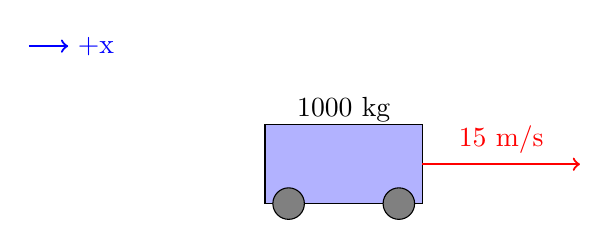
\begin{tikzpicture}
			
			% Draw the car
			\draw[fill=blue!30] (0,0) rectangle (2,1); % Car body
			\draw[fill=gray] (0.3,0) circle (0.2); % Rear wheel
			\draw[fill=gray] (1.7,0) circle (0.2); % Front wheel
			\node at (1, 1.2) {1000 kg}; % Car mass label
			
			% Draw the speed arrow
			\draw[->, thick, red] (2,0.5) -- (4,0.5) node[midway, above] {15 m/s};
			
		\draw[->, thick, blue] (-3,2) -- (-2.5,2);
				\node at (-2.5, 2)[blue, right] {+x}; % Car mass label
			
		\end{tikzpicture}
		\end{center}
	
	Since we know both the mass and the speed of the object, we can use equation \eqref{eqn:kineticenergy} to solve the problem:
	
		\begin{equation*}
		K = \frac{1}{2}mv^2 = \frac{1}{2}(\SI{1000}{kg})(\SI{15}{m/s})^2 = \SI{225000}{J}
	\end{equation*}

	
			
	
		
	\end{mdframed}
	
	\subsection{Potential energy} \index{Potential Energy} \index{Energy, Potential}
	\gls{potentialenergy} is energy that is stored.  Though there are many forms of potential energy, we will concentrate on two forms of stored energy in this section: gravitational potential energy and elastic potential energy.  In this text, potential energy is symbolized by the variable $U$, though it is quite common to find potential energy symbolized by the letters $PE$ as well. 
	
	A common misconception is that kinetic energy and potential energy cannot exist at the same time.  This is not the case, and object often have both kinetic energy and potential energy simultaneously.

	\subsubsection{Gravitational Potential Energy} \index{Gravitational Potential Energy} \index{Potential Energy, Gravitational} \index{Energy, Gravitational Potential}
	\gls{gravitationalpotentialenergy} is energy that is stored due to the interaction of an object with gravitational field.  When a relatively small object is in a uniform gravitational field (such as near the surface of a planet), the gravitational potential energy is given by: 
			\begin{mdframed}[backgroundcolor=orange!20!white]
		\begin{equation}
		U_g = mgh
		\label{eqn:gravitationalpotentialenergy}
		\end{equation}
	\end{mdframed}
	
	
 	\begin{mdframed}[backgroundcolor=blue!10!white]
 	\begin{center}
 		
 		
 		\textbf{Example \thesection.1}	
 	\end{center}
 	
 	\textbf{Problem: } A 2 kg block is held 3 meters above the ground. What is the gravitational potential energy of the block?
 	\vspace{0.1in}
 	
 	\textbf{Solution:} 
 	Begin by drawing a diagram:
 	\vspace{0.1in}
 	\begin{center}
 		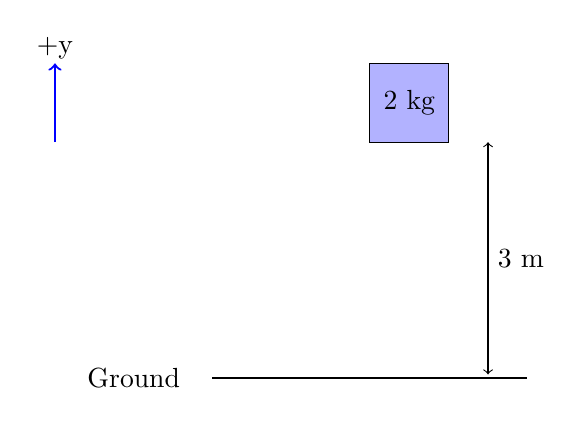
\begin{tikzpicture}
 			
 			% Draw the ground line
 			\draw[thick] (-1,0) -- (3,0); % Ground line
 			\node at (-2,0) {Ground};
 			
 			% Draw the block positioned above the ground
 			\draw[fill=blue!30] (1,3) rectangle (2,4); % Block as a rectangle
 			\node at (1.5,3.5) {2 kg}; % Label for block
 			
 			% Draw the height indicator
% 			\draw[dashed] (2,3) -- (2,0); % Dashed line to indicate height
 			\draw[<->] (2.5,0.05) -- (2.5,3) node[midway, right] {3 m}; % Height label
 			
 			% Draw the gravitational force arrow
 %			\draw[->, thick, red] (1.5,3) -- (1.5,1.5) node[midway, left] {$F_g = mg$}; % Gravity force arrow
 			\draw[->, thick, blue] (-3,3) -- (-3,4);
 			\node at (-3,4.2) {+y};
 		\end{tikzpicture}
 		
 		We can now calculate potential energy using equation \eqref{eqn:gravitationalpotentialenergy}:
 		
 		\begin{equation*}
 			U_g = mgh = (\SI{2}{kg})(\SI{9.81}{\frac{m}{s^2}})(\SI{3}{m}) = \SI{58.86}{J} 
 		\end{equation*}
 		
 	\end{center}
 	
\end{mdframed}
 	
	
	
	
	\subsubsection{Elastic Potential Energy} \index{Elastic Potential Energy} \index{Potential Energy, Elastic}
	
	\index{Potential Energy, Gravitational}
	Springs and other stretchable materials that return to their original shape when not subjected to external forces store \gls{elasticpotentialenergy}.  For an ideal spring, the force the spring exerts is proportional to the distance it has been stretched.  This is called \gls{hookeslaw}: 
	
		\begin{mdframed}[backgroundcolor=orange!20!white]
		\begin{equation}
		\overrightarrow{F_s} = -k\vec{x}
		\label{eqn:hookeslaw}
		\end{equation}
	\end{mdframed}
	where $k$ is the \gls{springconstant}, \index{Spring Constant}  and $x$ is the distance the spring has been stretched or compressed from its equilibrium position.
	
	Some calculus can show that the energy stored in a spring that obeys Hooke's Law is: 
	
	\begin{mdframed}[backgroundcolor=orange!20!white]
		\begin{equation}
		U_s = \frac{1}{2}kx^2
		\label{eqn:elasticpotentialenergy}
		\end{equation}
	\end{mdframed}

	While all real springs convert mechanical energy into heat when stretching or compressing, the amount of energy lost as heat (a process called hysteresis) is usually negligible.  However, some stretchable objects, such as rubber bands, lose significant amounts of energy as heat.  Thus, equations \ref{eqn:hookeslaw} and \ref{eqn:elasticpotentialenergy} are not applicable to these objects.  
	
	
		
	\begin{mdframed}[backgroundcolor=blue!10!white]
		\begin{center}
			
			
			\textbf{Example \thesection.1}	
		\end{center}
		
		\textbf{Problem: } Spring is streched a distance of 0.2 m using a force of 20 N.  
		\begin{enumerate}[label=(\alph*)]
			\item What is the spring constant of the spring?
			\item What is the elastic portential energy stored in the spring?
		\end{enumerate}
		\vspace{0.1in}
		
		\textbf{Solution:} 
		Begin by drawing a diagram:
		\vspace{0.1in}
		\begin{center}
			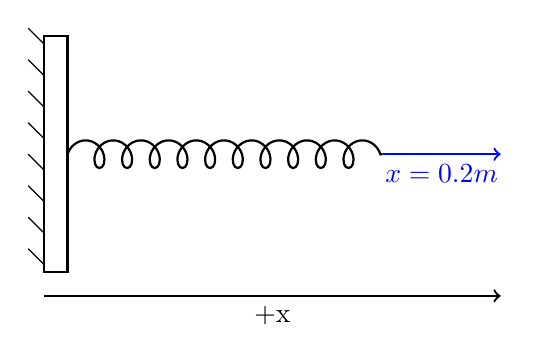
\begin{tikzpicture}
				% Draw a fixed wall
				\draw[thick] (0,0) -- (0,-1.5) -- (-0.3,-1.5) -- (-0.3,1.5) -- (0,1.5) -- cycle;
				\foreach \y in {-1.4,-1.0,...,1.4}
				\draw (-0.3,\y) -- (-0.5,\y+0.2);
				
				% Draw the spring
				\draw[thick,decorate,decoration={coil,aspect=0.8,amplitude=5pt,segment length=10pt}] (0,0) -- (4,0);
												
				
				% Add labels
				\draw[->,thick,blue] (4,0) -- (5.5,0) node[midway,below] {$x=\SI{0.2}{m}$};
				\draw[->,thick] (-0.3,-1.8) -- (5.5,-1.8) node[midway,below] {+x};
			\end{tikzpicture}
			
		
		\end{center}
		
		It should be noted that $F_s$ is the force exerted \textit{by} the spring, which is directed to the left in the diagram above.  Therefore, $F_s = \SI{-20}{N}$.  
\begin{enumerate}[label=(\alph*)]
	\item To find the spring constant, we can use Hooke's Law, Equation \ref{eqn:hookeslaw}:
	
		\begin{equation*}
			\overrightarrow{F_s} = -k\vec{x} \longrightarrow k = - \frac{\overrightarrow{F_s}}{\vec{x}} = -\frac{\SI{-20}{N}}{\SI{0.2}{m}} = \SI{100}{N/m}
		\end{equation*}
	
	\item Now that the spring constant is known, we can use equation \ref{eqn:elasticpotentialenergy} to find the elastic potential energy.  
	
			\begin{equation*}
		U_s = \frac{1}{2}kx^2 = \frac{1}{2}(\SI{100}{N/m})(\SI{0.2}{m})^2 = \SI{2}{J}
	\end{equation*}
\end{enumerate}
		
		
		
		
		
	\end{mdframed}
	
	
	
	
	\section{Work} 
\index{Work}
\gls{work} is the amount of energy that is transferred into or out of an object due to the application of a force that results in a displacement.  The formula for work is:

\begin{mdframed}[backgroundcolor=orange!20!white]
	\begin{equation}
		W = \vec{F}\cdot\vec{d}  
		\label{eqn:work}
	\end{equation}
\end{mdframed}

Note that both force and displacement are vectors, and work is the dot product of the two vectors.  Thus, referencing equation \ref{equation:dotproduct}
\begin{mdframed}[backgroundcolor=orange!20!white]
	\begin{equation}
		W = \vec{F}\cdot\vec{d}  = |\vec{F}| |\vec{d}| cos (\theta)
		\label{eqn:workdotproduct}
	\end{equation}
\end{mdframed}	
It should also be noted that for work to be done, there must be a non-zero displacement.  No work is done on an object that does not move.  




	\begin{mdframed}[backgroundcolor=blue!10!white]
	\begin{center}
		
		
		\textbf{Example \thesection.1}	
	\end{center}
	
	\textbf{Problem: } A person pulls a 10-kg sled along a flat surface by applying a force of 50 N at an angle of 30° above the horizontal. The sled moves a distance of 5 m. Assume there is no friction. How much work is done on the sled by the person?

	\vspace{0.1in}
	
	\textbf{Solution:} 
	Begin by drawing a diagram:
	\vspace{0.1in}
	\begin{center}
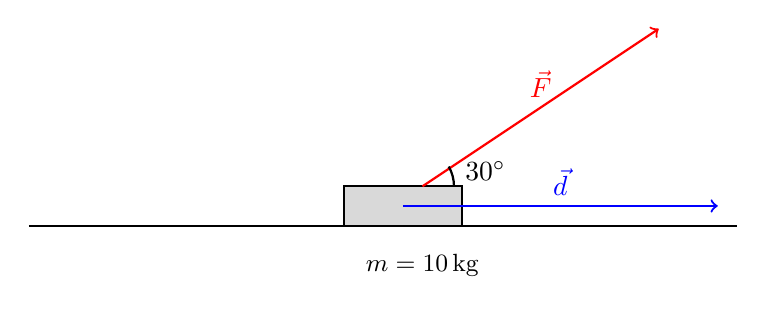
\begin{tikzpicture}
	% Draw the ground
	\draw[thick] (-1,0) -- (8,0);
	
	% Draw the sled
	\draw[thick,fill=gray!30] (3,0) rectangle (4.5,0.5);

	
	% Draw the force vector
	\draw[->,thick,red] (4,0.5) -- ++(3,2) node[midway,above] {$\vec{F}$};
	
	% Label the angle
	\draw[thick] (4.4,0.5) arc[start angle=0, end angle=30, radius=0.5];
	\node at (4.8,0.7) {$30^\circ$};
	
	% Draw the displacement vector
	\draw[->,thick,blue] (3.75,0.25) -- ++(4,0) node[midway,above] {$\vec{d}$};
	
	% Indicate mass of the sled
	\node at (4,-0.5) {\small $m = 10\,\mathrm{kg}$};
\end{tikzpicture}


		
		
	\end{center}
	
The work done on the sled can be found by applying equation \ref{eqn:workdotproduct}.


		\begin{equation*}
		W = \vec{F}\cdot\vec{d}  = |\vec{F}| |\vec{d}| cos (\theta) = (\SI{50}{N})(\SI{5}{m})cos(30 ^\circ) \approx \SI{216.506}{J}
	\end{equation*}
	
	
	
	
	
\end{mdframed}

	
	\section{The Work-Energy Theorem}
	The \textit{Work-Energy Theorem} states that doing work on an object causes that object's energy to change by the same amount as the work done.  This means that an object has 8 Joules of energy, and 2 Joules of work is done on the object, the object will have 10 Joules of work at the end of the process.  	While this is often associated with a change in kinetic energy, the energy change associated with work can also be associated with gravitational potential energy, thermal energy, or any other form of energy.  
	
		\begin{mdframed}[backgroundcolor=orange!20!white]
		\begin{equation}
			W = \Delta E
			\label{equation:workenergy}
		\end{equation}
	\end{mdframed}
	
		\section{Power}
	\index{Power}
	
	
	Power is defined as how quickly work is done.  Power is given by:
	
	\begin{mdframed}[backgroundcolor=orange!20!white]
		\begin{equation}
			P = \frac{W}{t}
			\label{equation:power}
		\end{equation}
	\end{mdframed}
	
	Since the work-energy theorem states that work is a change in energy, power is also used to describe how fast energy is flowing into or out of a system.
	
	\begin{mdframed}[backgroundcolor=orange!20!white]
		\begin{equation}
			P = \frac{\Delta E}{t}
			\label{equation:poweralt}
		\end{equation}
	\end{mdframed}
	

	
	
	\section{The Law of Conservation of Energy}
	\textit{The Law of Conservation of Energy} states that energy cannot be created or destroyed \footnote{This isn't entirely true.  This law will be tweaked in chapter \ref{chap:modern}.  }  This means that for a closed system, the total energy energy a system has in an initial state must be equal to the total energy in its final state.  Though the total energy must remain the same, this energy can change forms.  For instance, when a rock falls, gravitational potential energy turns into kinetic energy - but its total energy remains the same.  
	
	
	
	
	If, however, a system is open, and energy can flow into or out of the system, we must account for the energy that is either gained or lost.  Thus, a simple statement of the law of conservation of energy would be:
	
	
		\begin{mdframed}[backgroundcolor=orange!20!white]
		\begin{equation}
			E_i + \Delta E = E_f
			\label{equation:conservationofenergy}
		\end{equation}
	\end{mdframed}
	
	
	
	
	
	
	
	
	
	
	
	
	
	
	\newpage
	\section{Springs}
	
	We have already seen that springs follow Hooke's Law, given in equation \ref{eqn:hookeslaw}.  They also store elastic potential energy according to equation \ref{eqn:elasticpotentialenergy}.  When a spring is set into oscillatory motion, the period of \gls{oscillation} is given by the following formula.
	
		\begin{mdframed}[backgroundcolor=orange!20!white]
		\begin{equation}
		T_p = 2 \pi \sqrt{\frac{m}{k}}
		\label{eqn:springperiod}
		\end{equation}
	\end{mdframed}
	
	
	\begin{mdframed}[backgroundcolor=blue!10!white]
		\begin{center}
			
			
			\textbf{Example \thesection.1}	
		\end{center}
		
		\textbf{Problem: } A 0.25 kg mass is attached to a spring and set into oscillatory motion.  The period of the spring's motion is 0.45 seconds.  What is the spring constant of the spring? 
		
		\vspace{0.1in}
		
		\textbf{Solution:} 
		We can solve equation \ref{eqn:springperiod} for $k$ to answer this question.  
		
		\begin{equation*}
				T_p = 2 \pi \sqrt{\frac{m}{k}} \longrightarrow k = \frac{4\pi^2m}{{T_p}^2}  = \frac{4\pi^2(\SI{0.25}{kg})}{(\SI{0.45}{s})^2} \approx \SI{48.739}{N/m}
		\end{equation*}
		
		
		
		
		
	\end{mdframed}
	
	\section{Pendulums}
	A pendulum is any weight on the end of an arm that is free to swing back and forth.  You may have seen pendulums in old-fashioned clocks, and the swings at a park also act like a pendulum.  When a pendulum swings at a small angle ($\theta \lessapprox 5 \deg)$, the period of a pendulum is given by:
	
	\begin{mdframed}[backgroundcolor=orange!20!white]
		\begin{equation}
			T_p = 2 \pi \sqrt{\frac{l}{g}}
			\label{eqn:pendulumperiod}
		\end{equation}
	\end{mdframed}
	
	Notice that the period of a pendulum does not depend on the mass of the bob.  The only two variables that affect its period (assuming a small angle) are the length of the arm and gravity.  
	
	
	 
	

		


	


